%!TEX root = dippa.tex
%%% This file contains the Computational identification of microRNA targets section of my master's thesis.
%%% This section cover the computational methods for miRNA target identification.
%%% Author: Viljami Aittomäki

\section{Computational identification of miRNA targets}

% This section presents computational methods that have been used to predict
% putative target genes for microRNAs and regulatory networks between genes and
% microRNAs.

% Considering the recent large body of research on microRNAs, and their
% potential utility as biomarkers and treatment targets, it is not surprising
% that a plethora of computational tools have been released to aid in microRNA
% research.

% A recent review covering many published methods for different tasks
% has been written by Akhtar et al \citep{Akhtar2016}.

Recognizing the targets of microRNAs is essential in understanding their
biological function and role in disease. Many target
interactions have been found in experimental laboratory studies. Common
methods for such studies include using cell lines and introducing exogenous
miRNAs by transfection or suppressing endogenous ones and measuring the
effect on mRNA or protein expression. For a detailed review of experimental
methods, see Thomson et al \citep{Thomson2011}.

Several public databases list currently known experimentally validated
microRNA targets. Examples include DIANA-TarBase \citep{Vlachos2015} and
mirTarBase \citep{Chou2016}, which are both manually curated from published
literature, and MiRWalk \citep{Dweep2015}, which combines data from several
other databases using text mining.

Although recent advances in high-throughput methodologies, such as CLIP-seq,
have significantly increased the scale of experimental studies, experimental
identification of microRNA targets remains laborious and costly, and many
methods still rely on computational processing of results \citep{Vlachos2015}. To
this end, a wide range of computational tools have been developed to aid in
miRNA target discovery.

Computational approaches to target prediction can be roughly classified into
solely sequence-based tools and tools based on analysis of expression data
(which often incorporate sequence-based predictions). This section presents an
overview of published methods developed for target prediction.
Examples of these methods are shown in Table \ref{table:prediction-methods}.
For more in-depth reviews, see references \citep{Muniategui2013,Yue2009}.


\begin{table}
  \caption{Examples of tools for computational prediction of miRNA targets. All listed methods,
  except MAGIA, account only of suppression by miRNAs. \\
  Method: type of inference method used for predictions. \\
  SVM: support vector machine. HMM: hidden Markov model. MI: mutual information. \\
  Seq. used: sequence features considered (sequence-based methods) or use of
  previous sequence-based predictions (expression-based methods); see text for more details. \\
  i: sequence matches between the seed region and 3' UTR,
  ii: sequence matches outside the seed region (in the 3' UTR),
  iii: sequence matches in the 5' UTR or coding sequence of the mRNA,
  iv: free energy of the bound miRNA-mRNA duplex,
  v: evolutionary conservation of matches between species. \\
  prefilter: sequence-based predictions used as a filter prior to analysis. \\
  prior: sequence-based predictions included in prior distributions
  }
  \label{table:prediction-methods}
  %\centering
  {\fontfamily{lmss}\fontsize{10pt}{13pt}\selectfont
  \begin{tabular}{ lp{3cm}lp{5cm} }
    %\\[-1ex] \hline\hline
    \hline
    \textbf{Name} & \textbf{Method} & \textbf{Seq. used} & \textbf{Additional notes} \\
    \hline \\
    \multicolumn{4}{l}{\textbf{Sequence-based methods}} \\
    \\[-.3cm]
    TargetScan \citep{Agarwal2015}  & rule based            & i,ii,iv,v     & Originally the first published target prediction tool. \\
    miRanda \citep{Betel2008}       & rule based            & i,ii,v        & Aligns whole miRNA to mRNA 3' UTR. \\
    mirTarget \citep{Wang2008}      & SVM                   & i,ii,iii,iv,v &  \\
    rna22 \citep{Miranda2006}       & Markov chain and rule & i,ii,iv       & Uses a Markov chain to identify potential regions in mRNA 3' UTR and then sequence-rule filtering. \\
    PicTar \citep{Krek2005}         & rule and HMM          & (i, iv,v)      & Semi-supervised-like approach; uses strict sequence rules$^{\textup{i,iv,v}}$ to obtain a training set for a HMM classifier. \\
    TargetBoost \citep{Saetrom2005} & genetic \mbox{programming} & learned  & Learns sequence features and classifier from training data. \\
    \\
    \multicolumn{4}{l}{\textbf{Expression-based methods}} \\
    \\[-.3cm]
    MAGIA \citep{Sales2010}               & correlation, MI               & prefilter & Also produces a bipartite network of miRNA-mRNA interactions. \\
    TaLasso \citep{Muniategui2012}        & lasso \mbox{regression}       & prefilter &  \\
    Engelmann et al \citep{Engelmann2012} & least angle \mbox{regression} & none/prefilter & Least-angle regression is a specific implementation of lasso. \\
    miRNAmRNA \citep{vanIterson2013}      & global test                   & prefilter   & Uses mRNA expression profiles to predict miRNA expression. \\
    GenMir++/3 \citep{Huang2007,Huang2008}& Bayesian \mbox{regression}    & prefilter/i,iv,v & GenMir3 can incorporate sequence features into the model. \\
    Stingo et al \citep{Stingo2010}       & Bayesian \mbox{variable} \mbox{selection} & prior & Effectively a spike-and-slab variable selection approach, scores from any sequence-based method can be used as prior information. \\
    \hline
    \end{tabular}
    }
\end{table}




\subsection{Sequence-based target prediction}

Sequence-based prediction methods focus on finding miRNA-mRNA pairs that
have complementary sequences, as sequence complementarity
is the primary determinant of miRNA targeting.
% Hence, they can only determine pair-wise relationships.
From a machine learning perspective,
prediction of miRNA targets is essentially a \emph{classification}
problem, where the goal is to identify a set features (both of the miRNA and
mRNA) that allows classifying mRNAs as either a target or a non-target of any
given miRNA.

Most sequence-based approaches are essentially rule-based filters, where
features of both the miRNA and mRNA sequence are used to narrow down candidate
target lists \citep{Yue2009}. These features are derived from earlier
experimental knowledge, and commonly used features include:
(i) sequence matches between the seed region of the miRNA and 3' UTR of the mRNA,
(ii) sequence matches outside the seed region (in the 3' UTR),
(iii) sequence matches in the 5' UTR or coding sequence of the mRNA,
(iv) free energy of the bound miRNA-mRNA duplex, and
(v) evolutionary conservation of matches between species.
Rule-based prediction methods are unsupervised, i.e. no training data is
used to form the classifier. Instead, the relevance of the used features is
decided by the method's authors. An example of a rule-based algorithm
is depicted in Figure \ref{fig:miranda-flow}.

\begin{figure}[htb]
  \centering
  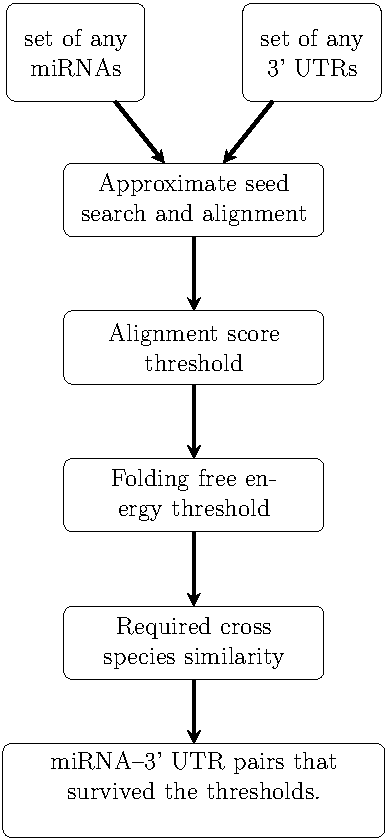
\includegraphics[width=0.3\linewidth]{figures/miRanda-flow.pdf}
  \caption{A schematic of the miRanda \citep{Betel2008} algorithm for
  miRNA target prediction. The algorithm takes as input a set of miRNA
  and mRNA sequences. It then searches the mRNA 3'UTRs for the seed sequence
  of each miRNA and performs an alignment of the miRNA and mRNA if the seed is found.
  Then thee free energy of the aligned miRNA-mRNA duplex is computed, and
  finally a conservation score between several species is computed for the
  aligned section of the mRNA. At each step a score threshold is used for
  filtering miRNA-mRNA pairs to the final set of candidate pairs.
  Modified with permission from \citep{Karhu2009}.}
  \label{fig:miranda-flow}
\end{figure}


% An example of a rule-based predictor is illustrated in Figure \ref{fig:rule-flow}.

Supervised machine-learning approaches has also been employed, where a
training data set consisting of experimentally validated targets and non-targets
(often obtained from expression data sets) is used to train a
classifier for classifying mRNAs as miRNA targets. Support vector machines (SVM)
are the most common choice for classifier. The features used for classification
are similar to rule-based tools, i.e. mostly derived from sequences, but supervised
learning allows the inclusion of much more features. For example mirTarget
uses a set of 113 features including seed region matches, conservation and a
range of different sequence features from different parts of the miRNA
sequence \citep{Wang2008}. More complex approaches have also been applied,
such as using genetic programming to learn sequence features, and using
Markov chains or hidden Markov models (HMM) as a sequence
generative model to estimate targeting probability.

% For a more thorough
% review of several different sequence features and algorithms using them,
% see the reviews by Yue et al \citep{Yue2009} and Bartel \citep{Bartel2009}.

The advantage of sequence-based methods is that they are based on
experimentally derived knowledge on molecular mechanisms and, thus, are likely
to represent causal relationships. As such, the predictions are easy to
interpret. Disadvantages of sequence-based methods include: considering only
pair-wise interactions cannot capture combinatorial effects; using sequence
conservation misses poorly conserved species-specific targets; requiring seed
region matches cannot identify miRNA targets without seed matches (while these
appear rare, they should not be discounted altogether \citep{Bartel2009}); a
sequence match does not always confer %\citep{Grimson2007}
repression and could be functionally inactive; and, finally, rule-based
methods are static and do not account for differing miRNA and mRNA expression
profiles in various tissues and disease states. There is also a general lack
of overlap between predictions from different sequence-based approaches,
suggesting that many results are spurious false positives
\citep{Muniategui2013}.




\subsection{Expression-data-based target prediction}\label{expr-methods}

Integrating expression data with sequence-based target prediction helps combat
the high false-positive rate of sequence-only methods and, importantly,
enables tissue and disease specific support for target predictions in real-world
data. Recent evidence indicates that miRNAs act predominantly through
mRNA degradation \citep{Guo2010}. Thus, it is feasible to use mRNA or protein
expression data to infer target relationships, since the regulatory effect of
miRNAs should be reflected in mRNA and protein abundances. Sequence-based
predictions are often incorporated as a preliminary filter step to limit the
potential interactions examined.

Various mathematical approaches, ranging from correlation to complex Bayesian
models, have been proposed for expression-based prediction. Most
methods limit the studied relationship to repression by the miRNA. This has
been suggested to improve performance \citep{Muniategui2012}, but has the
limitation of not being able to detect positive regulation, both direct and
indirect (mediated through regulation of other mRNAs) \citep{Engelmann2012}.
Notably, the majority of published efforts use either protein or mRNA 
expression together with miRNA expression, very few have combined all three.

% Mathematical models used in such expression
% analyses range from simple similarity measures to regression and complex
% Bayesian models, and examples are covered in this and the next section.

% Expression-based prediction methods use mathematical models that range from correlation
% to complex Bayesian regression models. The idea is to find (negatively)
% correlating miRNA-mRNA pairs or to predict mRNA or protein expression
% from miRNA expression patterns using regression. In the case of multiple regression
% target prediction becomes essentially a variable selection, where 
% the goal is to select microRNAs that best predict mRNA expression and then
% classify the mRNA in question as a target of chosen miRNAs.

Let us henceforth define $y_k = [y_{1k}, \dotsc y_{nK}]$ as a vector of expression
values of mRNA $k (k = 1, 2, \dotsc, K)$ and $X_{n \times p} = [x_j] =
[x_{ij}]$ as the matrix of expression values of miRNAs $j (j = 1, 2, \ldots,
p)$ for observations $i (i = 1, \ldots, n)$.

\paragraph{Correlation}
Several methods and publications use a straightforward approach to identifying
miRNA targets by finding miRNA-mRNA pairs whose expression patterns are
similar across observations. This is achieved with simple measures of variable
association. Pearson correlation is widely used because of its simplicity
and intuitive interpretation. Pearson correlation between mRNA $k$ and miRNA
$j$ is defined as:
\begin{equation}
	\rho_{kj} = (y_k)_{\mu_k=0|\sigma_k=1}^T \cdot (x_j)_{\mu_j=0|\sigma_j=1},
	\label{eq:pearson}
\end{equation}
where $\mu=0|\sigma=1$ indicates normalization to zero mean and unit
variance. Significantly correlated miRNA-mRNA pairs are classified as putative
target interactions. Other measures used include Spearman correlation and
mutual information (MI). A crucial limitation of correlation analysis is being
restricted to studying pair-wise associations. Single miRNAs often have a
small effect on mRNA expression, which leads to weak associations and,
therefore, low power to identify miRNA targets. This issue is worsened by a
large multiple-hypothesis testing problem when considering all possible miRNA-mRNA
pairs. Some approaches have used additional information, such as
sequence-based prediction or differential expression analysis, for limiting
examined miRNA-mRNA pairs to alleviate this to some extent
\citep{Muniategui2013}.
% The drawback of MI is that it only indicates similarity of the variables, but not
% the direction, or sign, of the relationship.

\paragraph{Multivariate linear regression}
Many proposed expression-based methods use some form of multivariate linear
regression (MLR) to examine the relationship between miRNAs and mRNAs.
Expression profiles of miRNAs are commonly used to predict the expression of a
single mRNA. Recently, Engelmann and Spang \citep{Engelmann2012} reported that miRNA expression can indeed be used to
predict mRNA expression. In the context of regression,
target prediction essentially becomes a \emph{variable selection} problem, where the
goal is to choose a set of miRNAs that best predict mRNA expression without
overfitting.

A linear regression model for the expression of mRNA $k$ is defined as
\begin{equation}
  \label{eq:linear-regression}
	y_k = \sum_{j=0}^{p} (\beta_{kj} \cdot x_j) + \epsilon_k =  X \beta_k + \epsilon_k,
\end{equation}
where $\beta_k = [\beta_{k0}, \dotsc, \beta_{kp}]$ is the vector of regression coefficients,
$\beta_{k0}$ is the intercept term, $\epsilon_k$ is the error term, and $X$ is the
matrix of covariates, i.e. the miRNA expression vectors (where a constant column
vector of $x_0=1$ has been added for the intercept). The parameter of
interest is $\beta_k$, which determines to the contribution of each miRNA to the
response variable $y_k$, i.e. mRNA expression. The regression error $\epsilon_k$
represents noise and fitting error caused by variation not captured by the
included covariates. $\epsilon_k$ is commonly assumed to be normally
distributed, with equal variance and no correlation between observations,
giving the \emph{normal linear model}. It is straightforward to incorporate previous
sequence-based predictions by adding an indicator variable $y_k = X c_k \beta_k + \epsilon_k$,
where $c_{kj} = 1$ if mRNA $k$ is a potential target of miRNA $j$, and $c_{kj} = 0$ otherwise.
% Commonly the solution is obtained by
% least squares, which involves minimizing the objective function,
% \begin{equation}
% 	min\{ || y_k - X \cdot \beta_k ||_2 \},
% \end{equation}
% which is equal to the sum of squares of the residuals.

The advantage of using regression for target prediction is the ability to
model the effect of several miRNAs on one gene simultaneously.
% This is desirable as the effect of a single
% miRNA on mRNA expression can be small, as discussed above.
Simple MLR is not applicable in cases, where the number covariates is larger
than the number of observations (here $p > n$)
\footnote{A characteristic that is very common
in analysis of high-throughput biological data, for example microarray
expression data.}, because the linear model is
undetermined and a single solution cannot be obtained.
Furthermore, simple MLR cannot solve the problem of
variable selection as the model fit improves asymptotically
by adding more covariates, leading to overfitting.

\paragraph{Regularized regression}
Both the dimensionality problem and overfitting can be overcome using regularized
regression. The most common approach is to apply regularized least squares,
where a penalty depending on the magnitude of the coefficients $\beta$
is applied to force them small. This entails minimizing the expression
\begin{equation}
	min\{ \left \| y_k - X \beta_k \right \|_2 + \lambda R(\beta_k) \} ,
\end{equation}
where the first term corresponds to fitting error (the sum of squared residuals),
$R(\beta_k)$ is the penalty function and $\lambda$ is a tuning
parameter that controls the amount of regularization. 
The 1-norm ($R(\beta_k) = \left \| \beta_k \right \|_1 = \sum_{j=0}^{j} \left | \beta_{kj} \right |$)
is frequently used for regularization; this is referred to as lasso regression
(shorthand for \emph{least absolute shrinkage and selection operator}).
% , where 
% regularizations include the 1-norm ($R(\beta) = ||\beta||_1$) in
% lasso regression, the 2-norm ($R(\beta) = ||\beta||_2$) in ridge
% regression and a combination of these ($R(w) =
% \lambda_1||\beta||_1 + \lambda_2||\beta||_2$) in what is called
% elastic-net regression.
Lasso regression in effect forces the number of non-zero coefficients in $\beta_k$
to be small, leading to a sparse solution that chooses seemingly important covariates.
% where as ridge regression results in a solution
% where coefficients are small but mostly non-zero \citep{Muniategui2013}.
While regularization solves the dimensionality problem and improves
interpretability, it has several important limitations. Firstly, regularization
may remove covariates highly associated with and functionally regulating the
response, instead retaining an unimportant covariate that correlates with
actual regulators \citep{Engelmann2012}. Secondly, only a limited number of
covariates may be included in the model, and thus some relevant associations
can be missed by number of included covariates alone. % \citep{vanIterson2013}.
Relating to both limitations, van Iterson et al \citep{vanIterson2013} showed that
lasso did not consistently select highly correlated miRNA-mRNA pairs.

\paragraph{Other approaches}
Other suggested approaches used include the global test \citep{vanIterson2013}, which is a
generalization for testing the global null hypothesis ($H_0: \beta = 0$) of a
linear regression model when $p >> n$, and approaches
similar to gene-set enrichment analysis, where the over-representation of
sequence-based target genes in differentially-expressed gene sets is considered
indicative of a target relationship in the studied condition. Le at al \citep{Le2015}
have proposed an ensemble
method, which combines predictions from several separate algorithms to build
on the advantages and compensate for the drawbacks of each.
Several Bayesian approaches have also been proposed; these are discussed in
the next section.


% A group of bioinformatics tools uses mRNA expression data to suggest
% potentially interesting miRNA-target interactions (MTIs).
% \begin{itemize}
%   \item
%   Input ist of interesting genes (e.g. DE vs normal)
%   \item
%   Look for miRNA regulation patterns in list (analogous to gene set enrichment REF REVIEW)
%   \item
%   Enriched miRNAs deemed interesting for this data
% \end{itemize}

% Ainakin nämä vaikka:
% \begin{itemize}
%   \item
%   DIANA-mirExTra (uusin versio NGS-datalle)
%   \item
%   GeneSet2miRNA
%   \item
%   Sylamer(?)
% \end{itemize}

% \paragraph{Correlation methods (incl MI)}\label{correlation-methods}

% Mutual information (MI) is a simple measure of similarity between two
% variables. \textbf{SELITÄ MI TARKEMMIN JA KAAVAN KANSSA JA LÄHDE} Thus, MI can
% be used to measure the interdependence of miRNA-mRNA pairs from expression
% data. However, MI does not distinguish the direction of the interaction, which
% is highly relevant for miRNAs that are believed to mostly downregulate mRNA
% expression. This constitutes a major drawback.
